
\chapter{Menu Scalars}\label{scalars_chapter}
\minitoc 

Simple numeric quantities (=numbers, or "scalar values") can be associated to each vertex of a given surface, and are referred to as "scalar arrays" in this section. 
As stated earlier, a given unselected surface can be colored using the currently active scalar array, if that surface contains that scalar array (see also Fig. \ref{4color_modes}-B p.\pageref{4color_modes}). To do so, the \textbf{array} display mode button must be pressed (
\includegraphics[scale=0.7]{images/04/show_color_scale.png}), and a scalar array must be selected as the currently active array (ex:
\includegraphics[scale=0.5]{images/04/scalarcombo_scalar.png}). The way scalar arrays are translated into colors can be set up using color maps, also referred to as "Lookup tables" (LUT) or color transfer functions. 

\section{Open scalars window}
The "Scalars" window can be opened by clicking on "
\includegraphics[scale=0.7]{images/04/color_scale_edit.png}" (see Fig. \ref{scalar_rendering_options_window}).

\begin{figure}
  \centering
  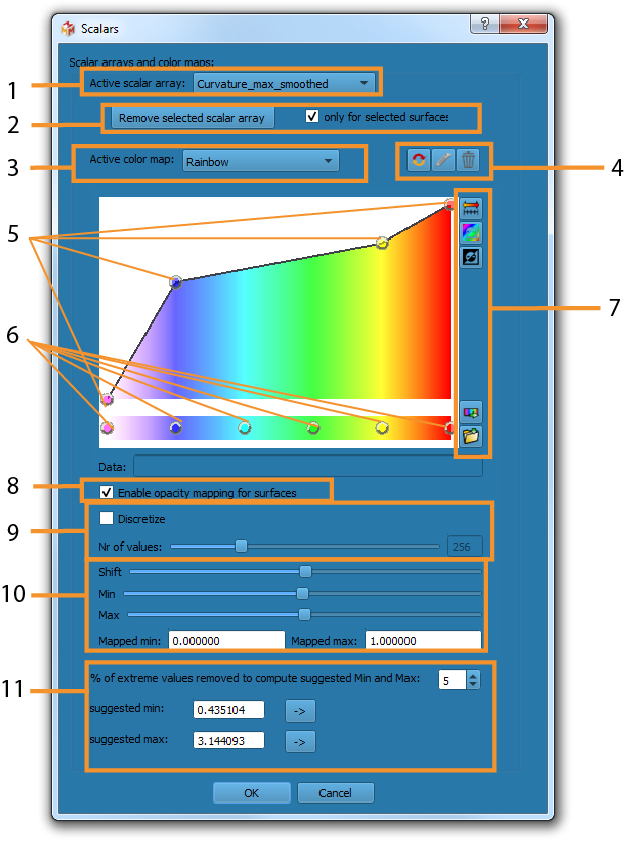
\includegraphics[scale=1]{images/11/scalar_rendering_option_window2.png}
\caption{Scalar control window. This window is divided in different subsections. \textbf{1)} choose current 3D rendered scalar array.  \textbf{2)} the active scalar array can be deleted from selected/all surface objects in this sections. \textbf{3)} choose current active color map, which transforms numbers into color and opacity on the screen. \textbf{4)} operations on the active colormap. a: reinitialize color map. b: export colors map(s) inside a .MAP file. c: change active color map name. d: delete active color map. \textbf{5)} opacity control points of the active color map. \textbf{6)} color control points of the active color map. \textbf{7)} modification controls of the active color map. a: set range to min and max. b: reverse color control points. c: reverse opacity control points. d: Save to preset = duplicate current active color map and create a new custom color map. \textbf{8)} enable/disable opacity mapping. \textbf{9)} discretize color levels, and choose number of levels. \textbf{10)} change min and max of color map. \textbf{11)} set min and max of color map based on suggested values. These suggested min and max values are computed in order to remove a percentage of most extreme minimal and maximal values found in the vertices of all opened surface for the active scalar.}	
\label{scalar_rendering_options_window}
 \end{figure}


\noindent
\textbf{\underline{Available controls:}}\\
\textbf{1: Active scalar array}: choose among the available scalars the one which will be displayed.\\\\
\noindent
\textbf{2: Remove selected scalar array}: deletes currently active scalar array from all opened surfaces, or  from selected surfaces only. This option is useful if you plan to save surfaces in the .vtk format and do not want MorphoDig to save associated scalar values (this will save some disk space).\\\\
\noindent
\textbf{3: Active color map}: choose among currently available colormaps. See Fig. \ref{change_active_color_map} for a practical example. \\\\

\begin{figure}
  \centering
  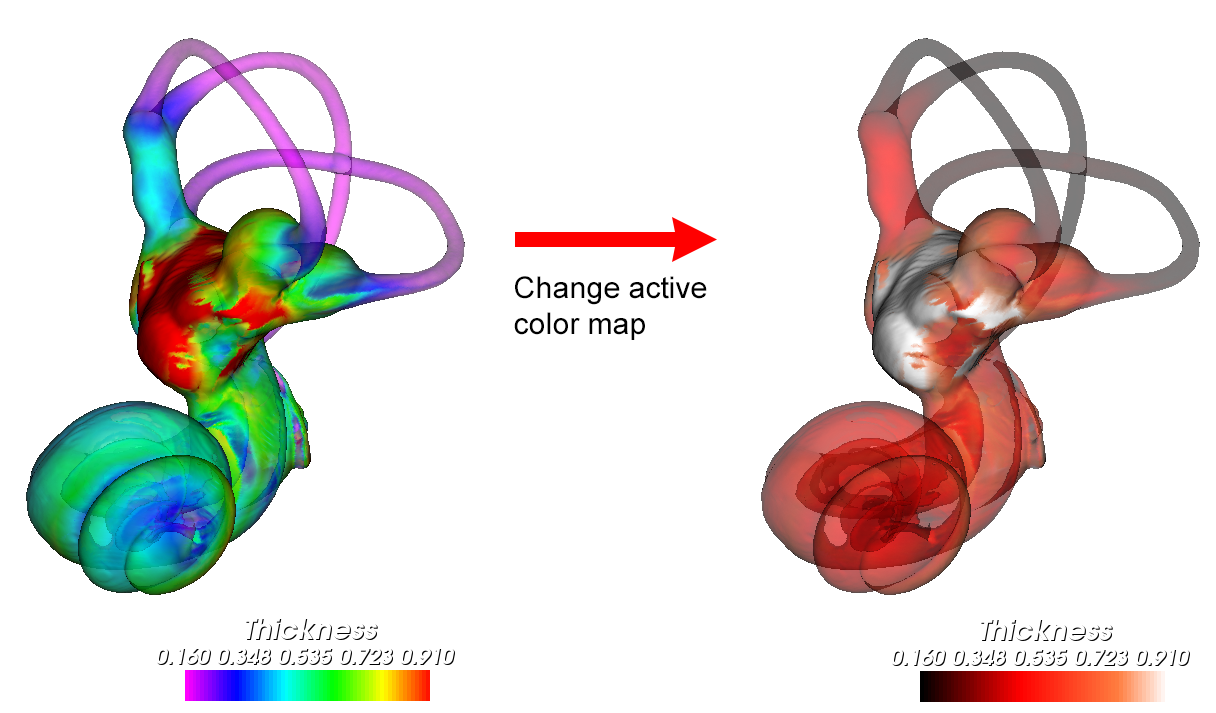
\includegraphics[scale=0.38]{images/11/change_active_color_map.png} 
	\caption{
Example of active colormap modification.  Left: left inner ear of \textit{Galago moholi}. Active scalars: thickness. Colormap: rainbow. Right: the same inner ear after the active colormap has been set to "Black-red-white".}
\label{change_active_color_map}
 \end{figure}


\noindent
\begin{minipage}{0.5\textwidth}
\textbf{4: Color map controls}: Four buttons are available. a:reinitialize color map (only possible for the 2 first predefined color maps). b: export color maps(s). When clicked, the export color map(s) dialog shows up (see Fig. \ref{export_color_maps}), in which you may define more precisely the color map(s) that should be exported.  c: change active color map name (can be only done on custom color maps). d: delete active color map (only custom color maps can be deleted).\\
\end{minipage}    
\begin{minipage}{0.5\textwidth}\centering
  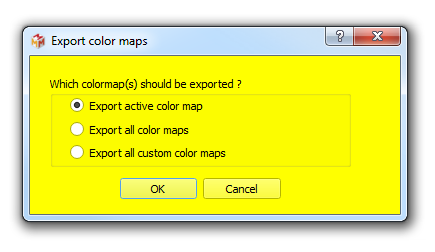
\includegraphics[scale=0.5]{images/11/export_color_maps.png}
 \captionof{figure}{Export color maps dialog.}
\label{export_color_maps}
 \end{minipage} \\\\

\noindent
\textbf{5: Opacity control points }: opacity control points of the active color map. Such control points can be added (left click on a line), deleted (select one control point using the left mouse button then press "delete") and edited (drag one control point using the left mouse button) interactively.\\\\

\noindent
\textbf{6: Color control points }: color control points of the active color map. Such control points can be added (left click on an empty zone), deleted (select one control point using the left mouse button then press "delete") and edited (drag one control point using the left mouse button) interactively.\\\\
\noindent
\textbf{7: additional color map controls}. From top to bottom. a: set colormap range to match the global active scalar min and max found for all currently opened surfaces. b: reverse color color control points (see Fig. \ref{invert_colors}). c: reverse opacity control points (see Fig. \ref{invert_opacities}). d:  Save to preset = duplicate current active color map and create a new custom color map.duplicate current active color map and create a new custom color map. \\\\



\begin{figure}
  \centering
  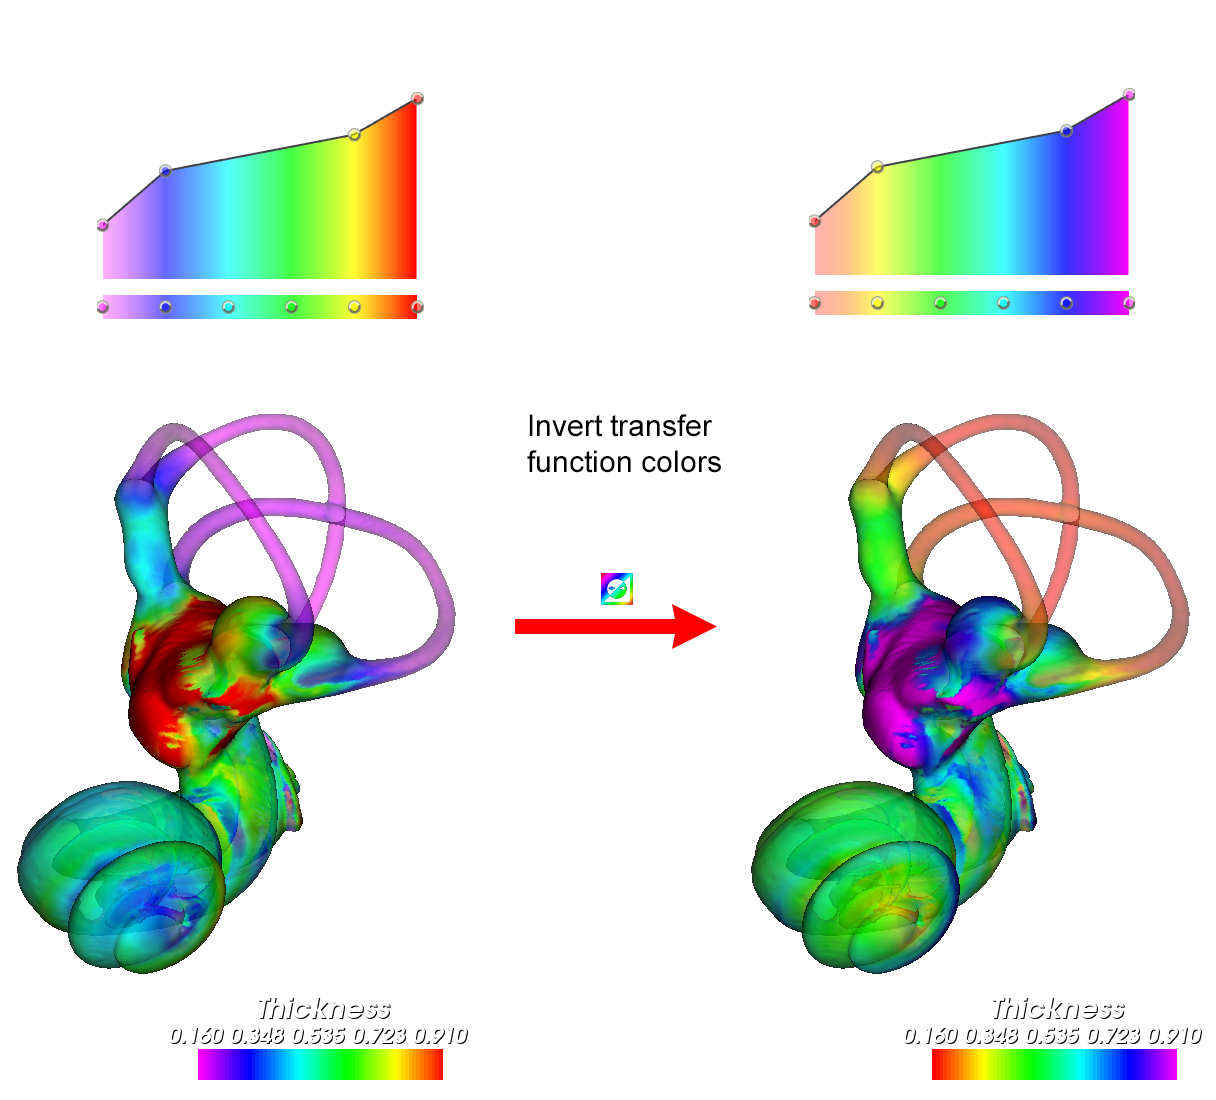
\includegraphics[scale=0.38]{images/11/invert_colors.png} 
	\caption{
Example of color inversion of a colormap.  Left: left inner ear of \textit{Galago moholi}. Active scalars: thickness. Colormap: rainbow. Right: the same inner ear after the color control points of the rainbow colormap have been reversed.}
\label{invert_colors}
 
\end{figure}

\begin{figure}
  \centering
  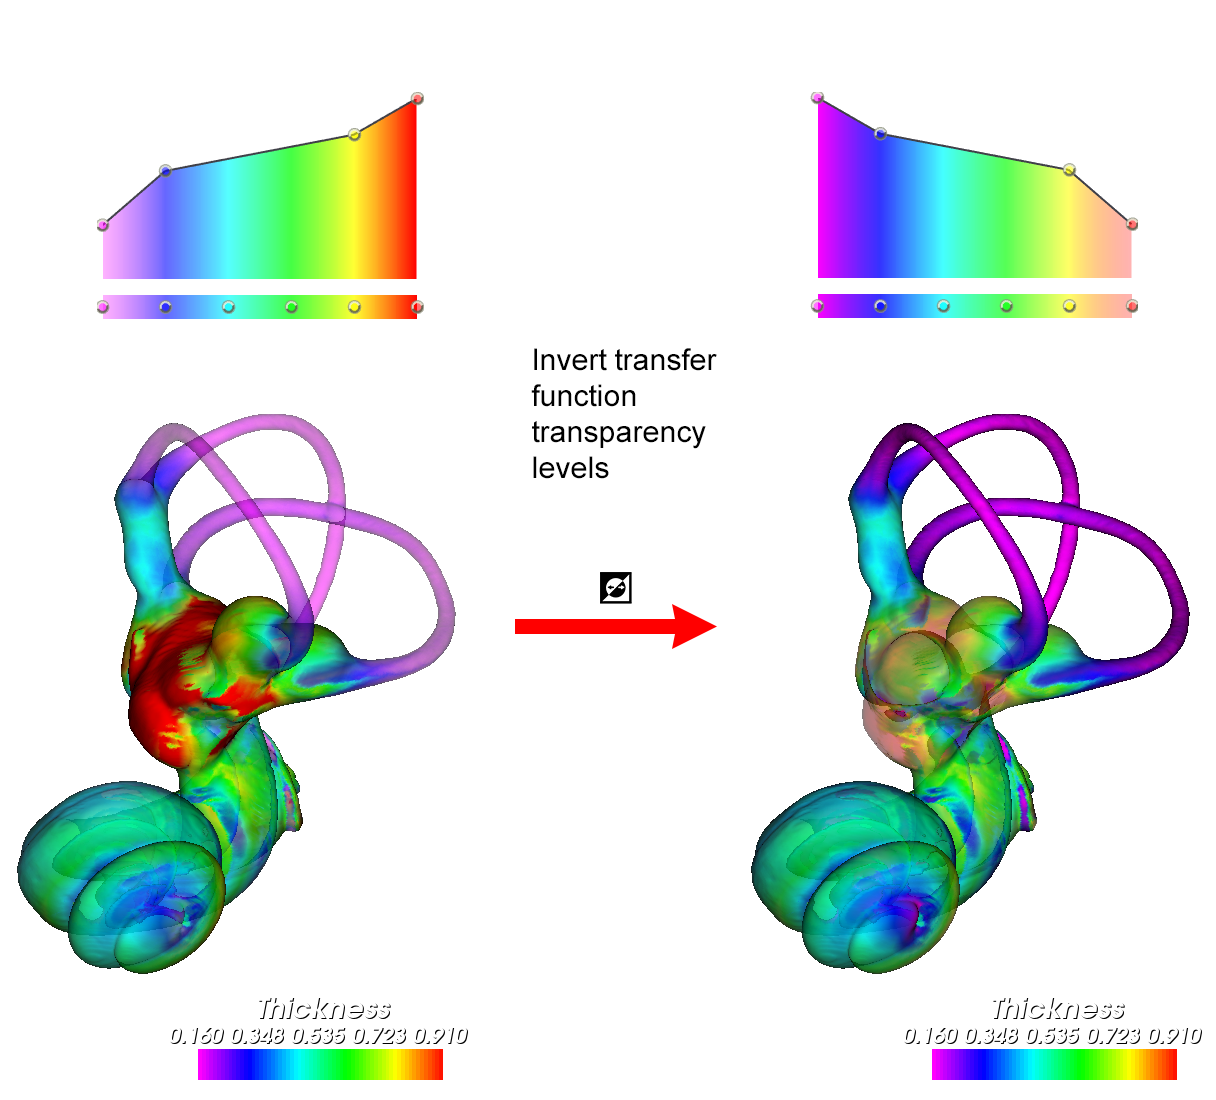
\includegraphics[scale=0.38]{images/11/invert_transparency.png} 
	\caption{
	Example of opcacity inversion of a colormap.  Left: left inner ear of \textit{Galago moholi}. Active scalars: thickness. Colormap: rainbow. Right: the same inner ear after the opacity leveles of the rainbow colormap have been reversed.}
\label{invert_opacities}
 
\end{figure}

\noindent
\textbf{8: enable/disable opacity mapping.} When opacity mapping is disabled, all surface objects are rendered using their "global" transparency level.\\\\

\noindent
\textbf{9: discretize color levels}, and choose number of levels. See Fig. \ref{discretize_example} for a practical example.\\\\
\begin{figure}
  \centering
  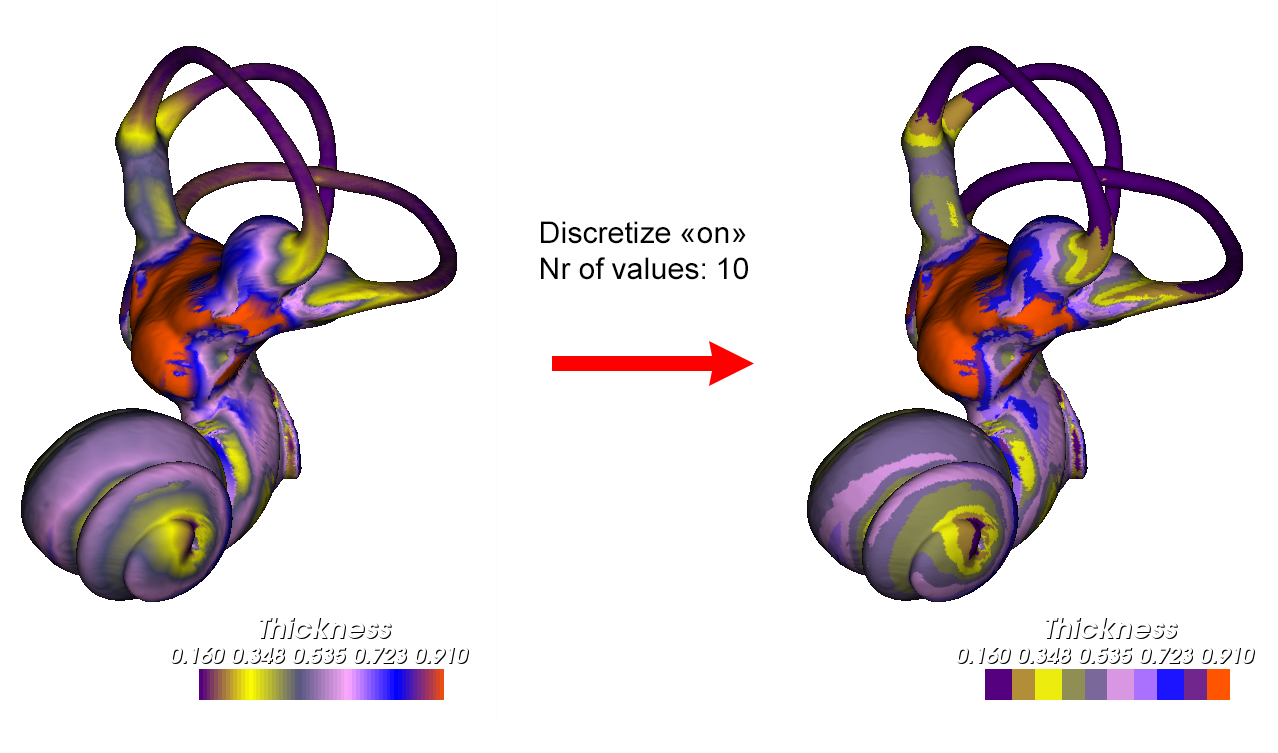
\includegraphics[scale=0.38]{images/11/discretize_on.png} 
	\caption{
Example of colormap discretization.  Left: left inner ear of \textit{Galago moholi}. Active scalars: thickness. Colormap: custom. Right: the same inner ear after the "discretize" option has been turned on, and the nr of values set to 10.}
\label{discretize_example}
 
\end{figure}

\noindent
\textbf{10: change min and max of color map.} You may use these sliders to change the minimal and maximal values of the active color map. By default, all colormaps range between 0 (min) and 1 (max), which may not be the most appropriate range to display a given scalar array. \\\\ 


\noindent
\textbf{11: set min and max of color map based on suggested values.} As stated above, by default, all colormaps range between 0 (min) and 1 (max), which may not be the most appropriate range to display a given scalar array. You may set the minimal and maximal values of the active colormap based on suggested values, which are computed automatically based on the currently opened surface objects, and which are computed in order to use the color scale at its best. See Fig. \ref{accept_suggested_min_max} for a practical example. \\\\

\begin{figure}
  \centering
  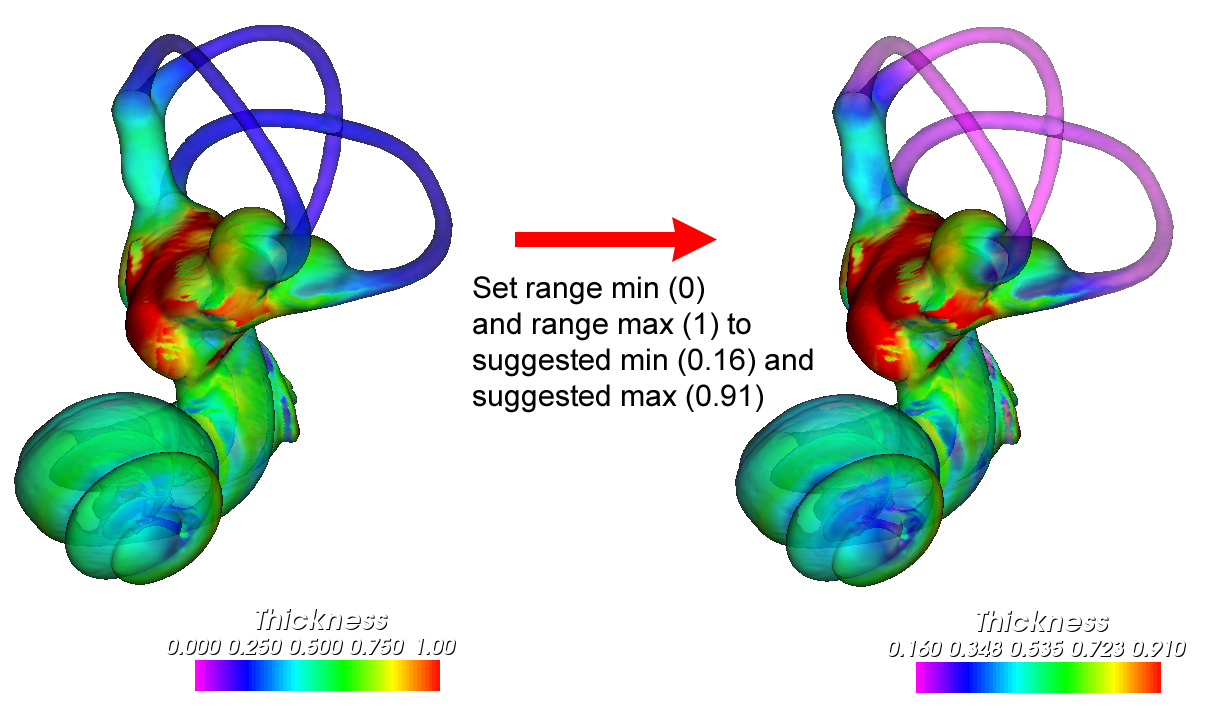
\includegraphics[scale=0.38]{images/11/accept_suggested_min_max.png} 
	\caption{
Example of suggested min and max usage. Left: Left inner ear of \textit{Galago moholi}. Active scalars: thickness. Colormap: rainbow. Te rainbow colormap is set as by default to range between 0 (min) and 1 (max). Right: the same inner ear after the rainbow colormap range has been modified based on suggested min (0.16) and suggested max (0.91) values.}
\label{accept_suggested_min_max}
 
\end{figure}
\noindent




\section{Compute distance from camera for each selected surface}
\noindent
Computes distance (=depth) from camera for all vertices of all selected surfaces. This option may offer a better
perception of the 3D structure of an object on a 2D screen representation. This option also makes it possible to compute an elevation map. See Fig. \ref{camera_distance} for a practical example. 
 
\begin{figure}
  \centering
  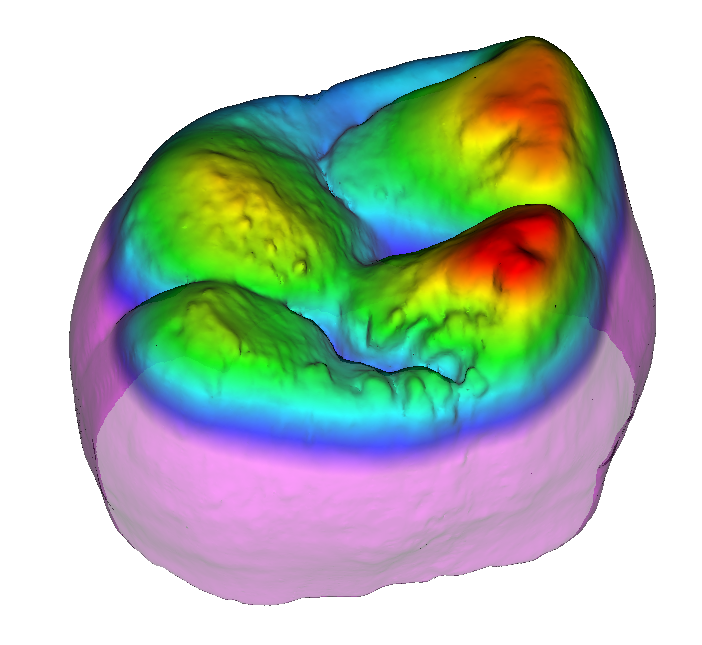
\includegraphics[scale=0.38]{images/11/camera_distance_example.png} 
	\caption{
Example of camera distance scalar array. Displayed specimen: upper outer enamel surface of a second upper molar of \textit{Homo sapiens}.}
\label{camera_distance}
 
\end{figure}
\noindent


\noindent



\section{Compute thickness within each selected surface}
\begin{minipage}{0.5\textwidth}
Thickness within an object (see Fig. \ref{thickness_within_dialog}) is defined the following way: for a
given vertex, the minimal distance between this vertex and other
vertices in the direction opposite to that of the surface's normal. In order to minimize computation time, a maximal
distance (Maximal thickness (size unit) ) is asked to the user, in order
to reduce the amount of vertices investigated at a given location. Also, in order to avoid to take into account only relevant vertices in that computation, an angular limit between investigated vertex normals (by default: 70\degree) is asked. Finally, a smoother scalar array output can be produced by setting the "thickness" value as the average of the distance found between a number of closest vertices found. See Fig. \ref{thickness_examples}-A for a practical example. 
 
\end{minipage}    
\begin{minipage}{0.5\textwidth}\centering
 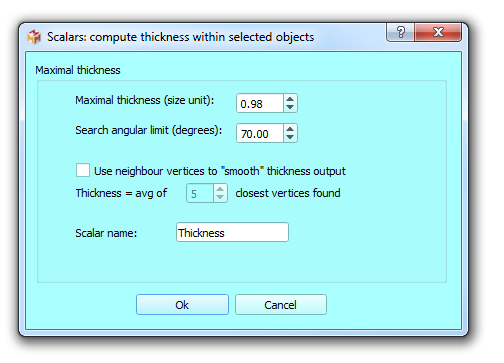
\includegraphics[scale=0.5]{images/11/thickness_within_dialog.png}
 \captionof{figure}{Thickness within a given surface.}
\label{thickness_within_dialog}
 \end{minipage} 


\begin{figure}
  \centering
  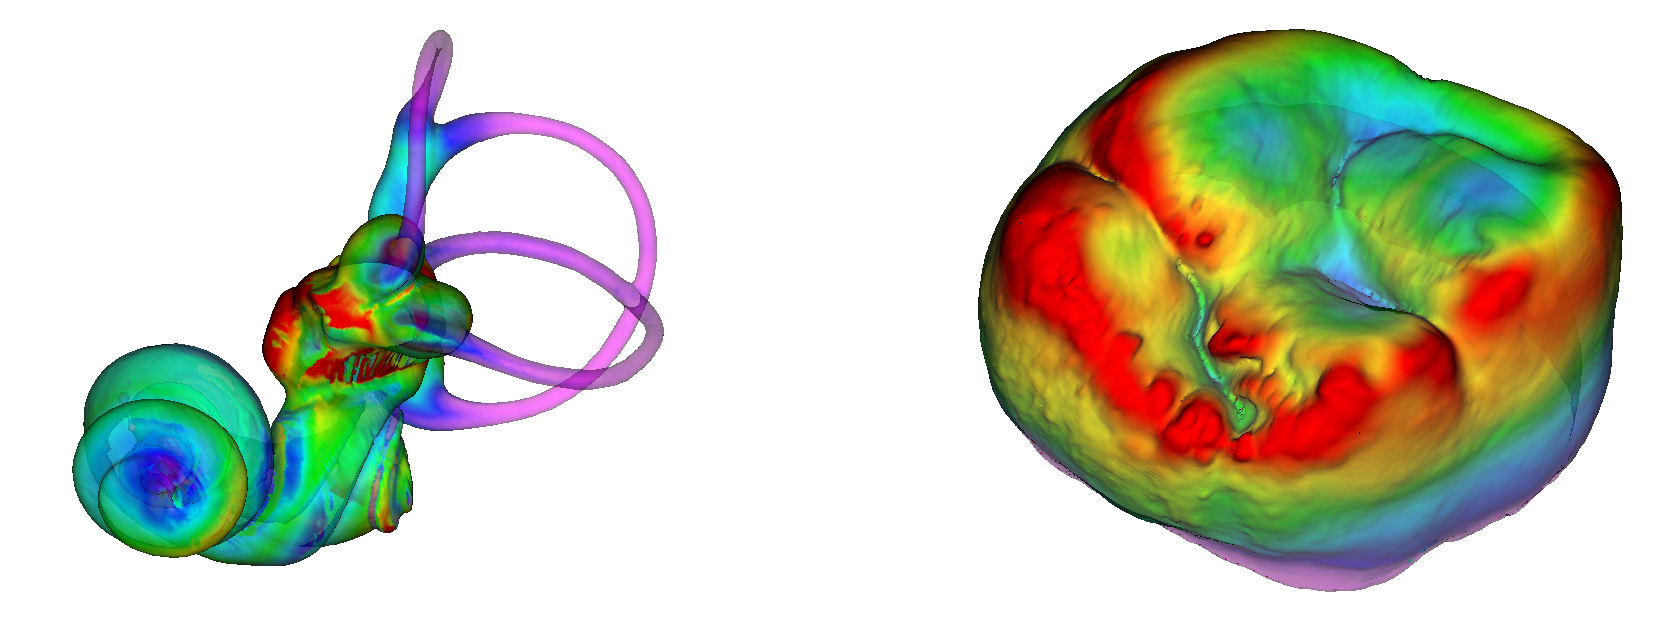
\includegraphics[scale=0.28]{images/11/thickness_examples.png} 
	\caption{
Examples of thickness computation. A: thickness within object. Specimen: left inner ear of \textit{Galago moholi}. B: thickness between the outer enamel surface (OEJ) and the enamel-dentine junction (EDJ) of a second upper molar of \textit{Homo sapiens}.}
\label{thickness_examples}
 
\end{figure}




\section{Compute thickness between two surfaces}

\noindent
\begin{minipage}{0.5\textwidth}
Thickness between two objects is defined the following way (see Fig. \ref{thickness_between_dialog}):
for a given vertex of the impacted object, the minimal distance
between this vertex and other vertices of the observed surface in
the same direction (if "invert normals of observed object" option is unchecked) or in the opposite direction (if "invert normals of observed object" option is checked) to that of the impacted surface's normal is computed. Again, in order to minimize computation time, a maximal distance (Maximal thickness (size unit) ) is asked to the user, in order to reduce the amount of vertices investigated at a given location. Also, in order to avoid to take into account only relevant vertices in that computation, an angular limit between investigated vertex normals (by default: 70\degree) is asked. Finally, a smoother scalar array output can be produced by setting the "thickness" value as the average of the distance found between a number of closest vertices found. See Fig. \ref{thickness_examples}-B for a practical example.
\end{minipage}    
\begin{minipage}{0.5\textwidth}\centering
  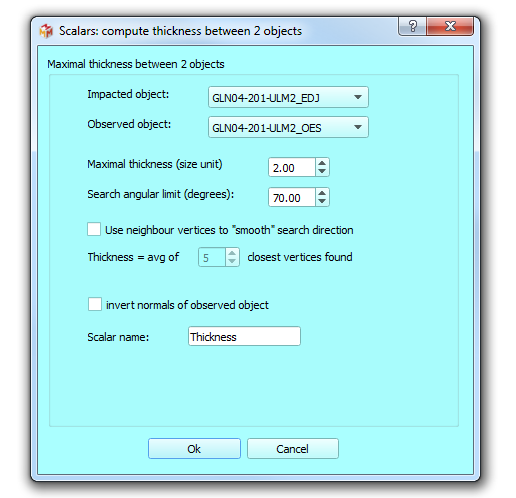
\includegraphics[scale=0.5]{images/11/thickness_between_dialog.png}
 \captionof{figure}{Thickness between 2 surfaces window}
\label{thickness_between_dialog}
 \end{minipage} 
\noindent


\section{Compute distance between two surfaces}
\noindent
\begin{minipage}{0.5\textwidth}
Vertex closest distance between two objects is computed as the minimal distance between all vertices  vertex and other vertices of the observed surface, regardless of the direction. This option may be relevant if you want to compare the same object twice (for instance the object before and after some alteration) or want to compare two objects of very similar shape (for instance two inner ears belonging to two specimens of the same species). Before computing a distance map, it is strongly advised, in a preliminary step, to align the two compared surfaces (see section \ref{surface_alignment_section} p.\pageref{surface_alignment_section}). The computed distance can be somewhat "smoothed" by being defined as the average value of a given number of closest vertices. Again, in order to minimize computation time, a maximal distance (in size unit) is asked to the user, in order to reduce the amount of vertices investigated at a given location. See Fig. \ref{distance_between_example} for a practical example.
\end{minipage}    
\begin{minipage}{0.5\textwidth}\centering
  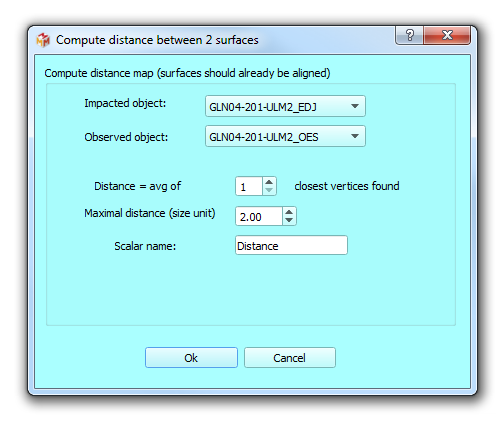
\includegraphics[scale=0.5]{images/11/distance_between_dialog.png}
 \captionof{figure}{Distance between 2 surfaces window}
\label{distance_between_dialog}
 \end{minipage} 
\noindent


\begin{figure}
  \centering
  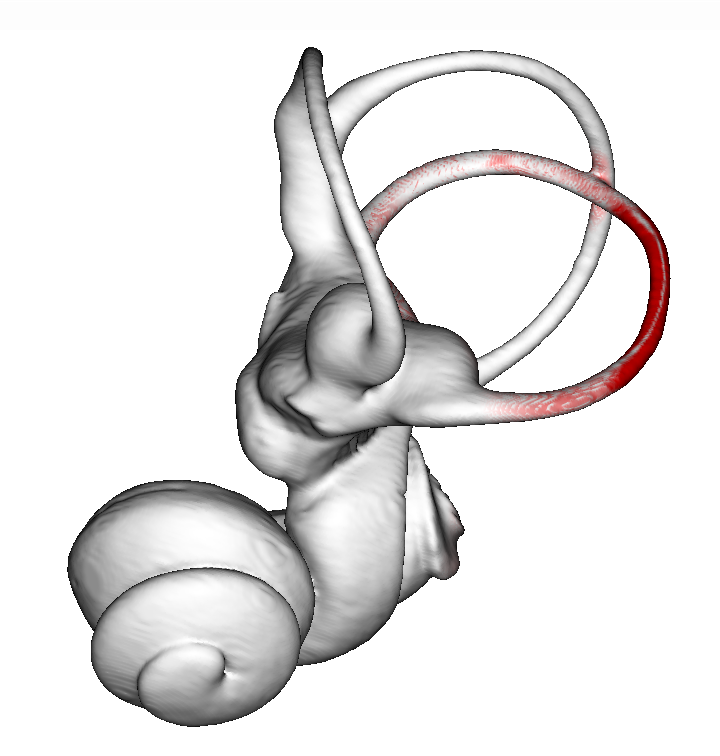
\includegraphics[scale=0.28]{images/11/distance_between_example.png} 
	\caption{
Example of distance map between two surfaces. An inner ear of \textit{Galago moholi} was virtually distorted in the lateral canal region. The corresponding representation of the deformation is shown here using a distance map: in red can we identify the most distorted regions.}
\label{distance_between_example}
 
\end{figure}



\section{Compute curvature for each selected surface}
\noindent
\begin{minipage}{0.5\textwidth}
Curvatures are computed using the vtkCurvatures filter.\\
vtkCurvatures filter offers 4 ways to compute surface's
curvature at each vertex (see Fig. \ref{curvature_example}):\\
- Principal maximal curvature\\
- Principal minimal curvature\\
- Gaussian curvature\\
- Mean curvature.\\
See vtkCurvatures' documentation for further details.

\end{minipage}    
\begin{minipage}{0.5\textwidth}\centering
  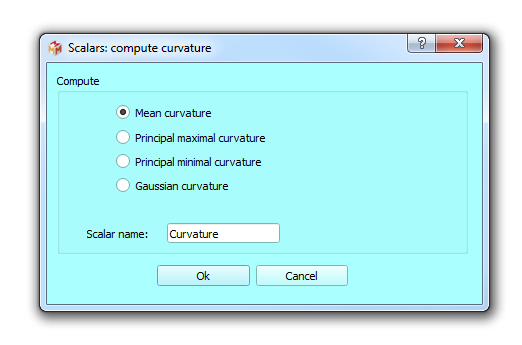
\includegraphics[scale=0.5]{images/11/curvature_dialog.png}
 \captionof{figure}{Curvature dialog}
\label{curvature_dialog}
 \end{minipage} 
\noindent

\begin{figure}
  \centering
  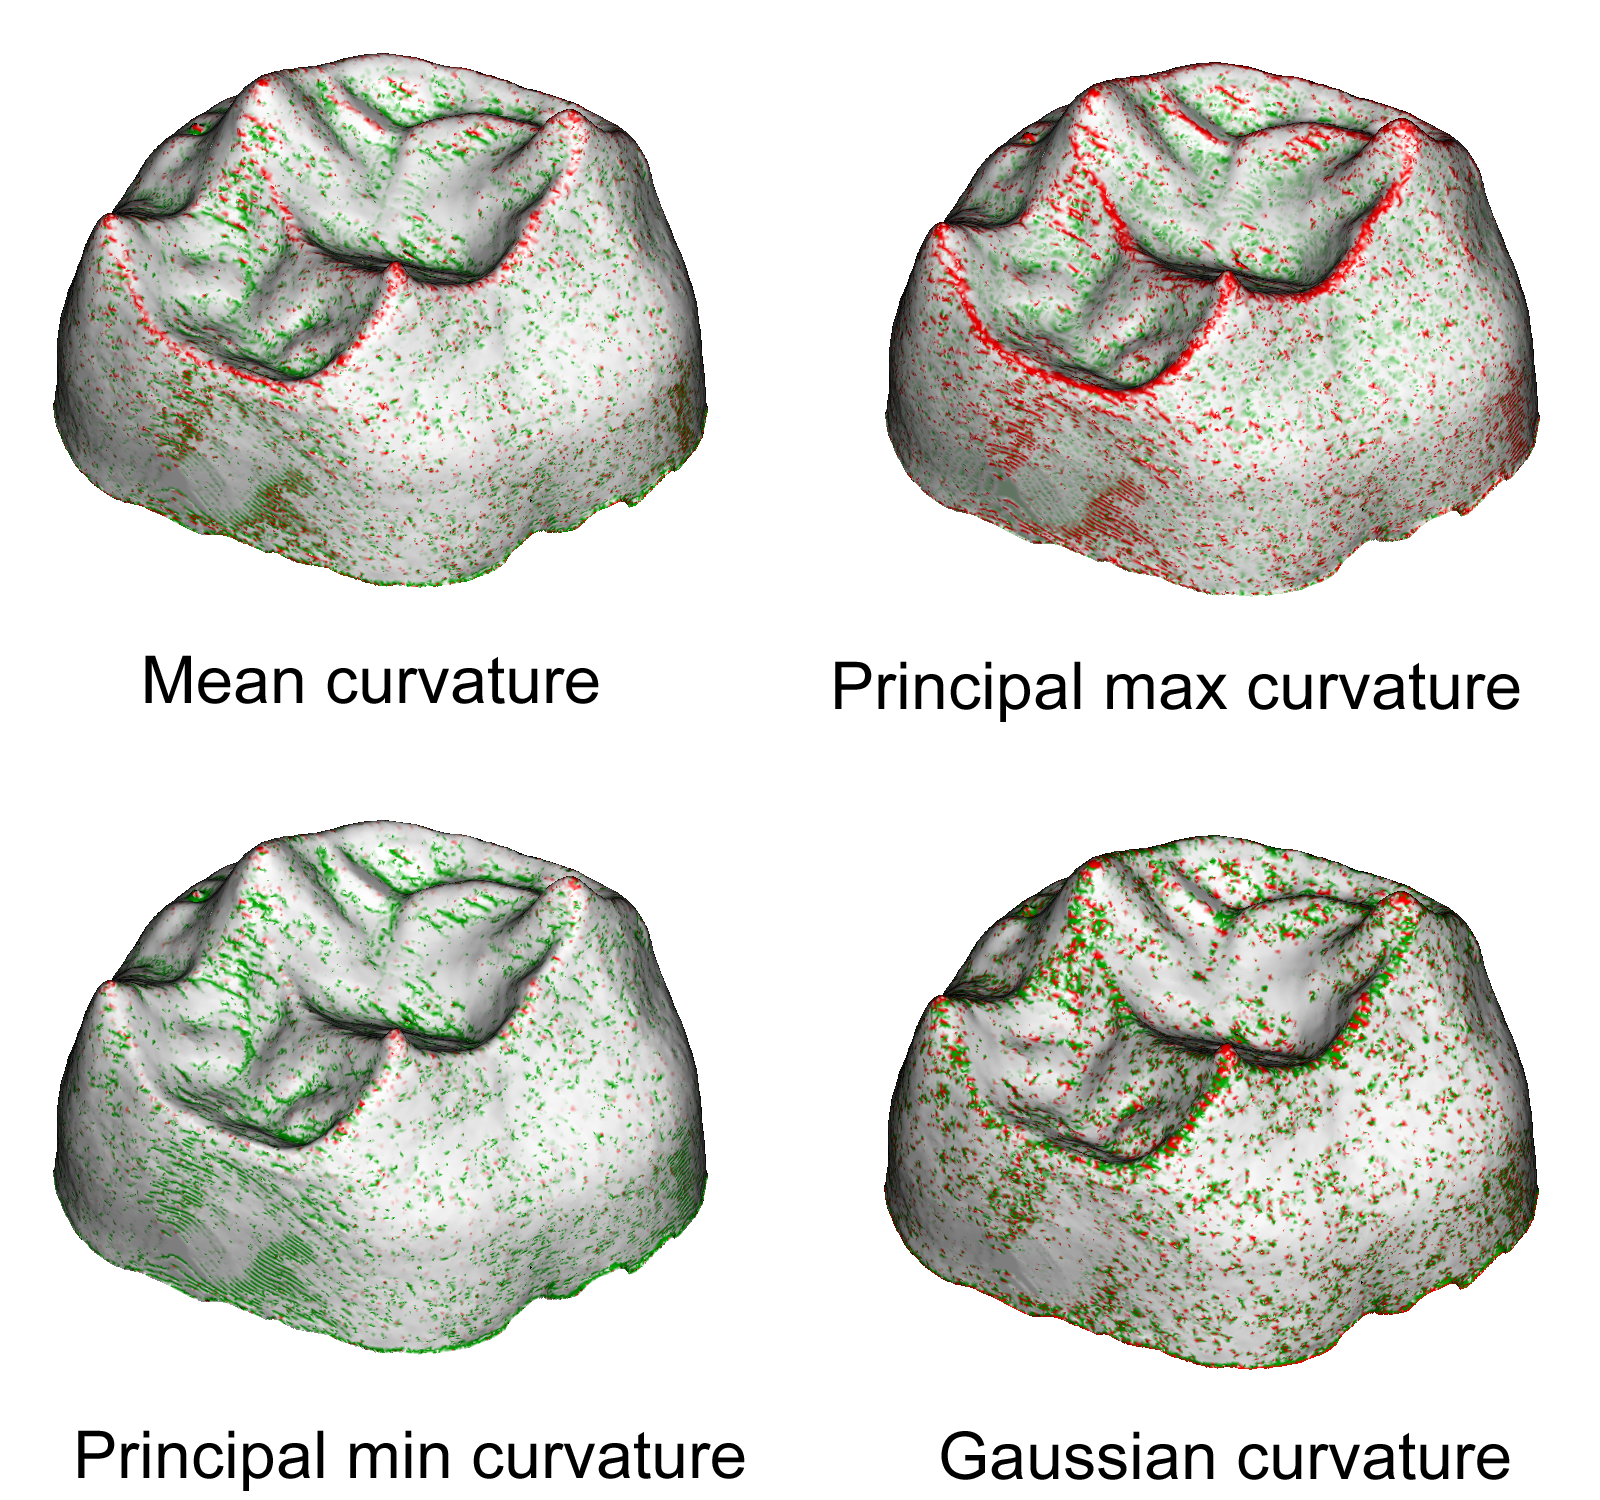
\includegraphics[scale=0.3]{images/11/curvature_example.png} 
	\caption{
Examples of 3D rendering of ``Curvature" scalars. Scalar mode is active, the rainbow color scale is used. Specimen: enamel dentine junction (EDJ) of the second superior molar of Neolithic human of the necropolis of Gurgy (France). Image credit: Mona Le Luyer.}
\label{curvature_example}
 
\end{figure}

\section{Compute complexity for each selected surface}
In section \ref{global_complexity_1} p.\pageref{global_complexity_1} and section \ref{global_complexity_2} p.\pageref{global_complexity_2}, proxies for shape complexity (= how much area can be enclosed within a given volume) are described. The limit of those approaches is that they produce single values for a whole surface, and do not take into account shape variation within surfaces. However, a single biological object can express a lot of shape variability. In this section, we extend the approach of shape complexity described earlier: we provide surface complexity measurements for all vertices of a surface. To do so, for each vertex, a local surrounding area is extracted and shape complexity is measured for this local area. The consequence of this approach is that these measurements depend on the extent of the local area investigated for each vertex. For a given surface, the "local" area investigated is a sphere of radius "R".  By default, for a given surface, R is computed as follows:
\begin{equation}
R = \dfrac{Avg(length(PC1)+length(PC2)+length(PC3)))}{18}
\end{equation}
 
The numerator of this equation is in our view a sensible estimate of the "average extension" of an object in 3D space. It is computed as is the average of the lengths of a given object along its 3 principal extension axes. This measurement is obtained  by performing a principal component analysis on the vertex coordinates of a given surface. The denominator (18) is set empirically, as it seems to provide a reasonable estimate of "locality" for all vertex locations, regardless the global shape of the investigated surfaces. However, R can be set to a custom value in the Scalars complexity dialog (see Fig. \ref{complexity_dialog}).

\begin{figure}
  \centering
  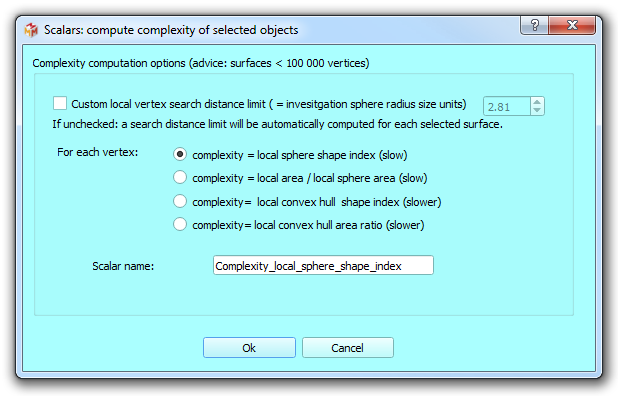
\includegraphics[scale=0.5]{images/11/complexity_dialog.png} 
	\caption{Complexity dialog.}
\label{complexity_dialog}
 
\end{figure}


Four complexity measurements are provided:

\subsection{Local Convex hull Area Ratio (LCh-AR)}
For each vertex V, the surrounding surface's local region enclosed within an area defined by a local sphere of center V and radius R is extracted. Then the local convex hull normalized area ratio (ChAR) is computed  for this  local region. ChAR is defined as the ratio between the extracted local surface area and the surface area of the convex hull computed for the same extracted local surface. \\
 This measurement of surface complexity takes more time to compute (computation of a Convex hull for each vertex) than the LS-AR and LS-NSI indices (see below) based on the local sphere, but it has two advantages (see Fig. \ref{complexityexample}-B p.\ref{complexityexample}):\\
- very low "border" artifacts (complex structures located at the outskirts of surfaces are given high complexity values).\\
- contrary to the LCh-NSI index (see below), isolated very flat (and non-complex) structures are given, as they should be, low complexity values .

\subsection{Local Sphere Area Ratio (LS-AR)}
For each vertex V, the surrounding surface's local region enclosed within an area defined by a local sphere of center V and radius R is extracted. Then complexity is computed as the ratio between the area of the extracted surface and the area of the sphere of radius R.   \\
This measurement of surface complexity takes less time to compute than the LCh-AR index, but it has one main drawback  (see Fig. \ref{complexityexample}-C p.\ref{complexityexample}):\\
- border artifacts: as the denominator used to construct this index is based on the surface area of the local sphere for a given vertex V, vertices located at the outskirts of a surface are given underestimated complexity values (and as a general rule, LS-AR tend to underestimate complexity in regions containing a small number of vertices) .

\subsection{Local Convex hull Normalized Shape Index (LCh-NSI)}
For each vertex V, the surrounding surface's local region enclosed within an area defined by a sphere of center V and radius R is extracted. Then the local convex hull normalized shape index (ChNSI) is computed  for this  local region (see section \ref{global_complexity_2} p.\pageref{global_complexity_2} for explanations of ChNSI index). \\
This measurement of surface complexity takes more time to compute (computation of a Convex hull for each vertex) than the LS-AR and LS-NSI indices (see above and below) based on the local sphere, but it presents one advantage over the LS-NSI: (see Fig. \ref{complexityexample}-D) p.\ref{complexityexample}:\\
- very low "border" artifacts (complex structures located at the outskirts of surfaces are given high complexity values).\\
However, this index has a considerable drawback: it produces overestimated complexity values for all very flat + very isolated areas (which are typically non complex areas). The reason is that the denominator used to construct this index is based on the surface volume of the local convex hull, which tends to be almost null for very flat and isolated areas. So if your structure presents such flat-and-isolated regions, we advise you not to use this index.

\subsection{Local Sphere Normalized Shape Index (LS-NSI)}
For each vertex V, the surrounding surface's local region enclosed within an area defined by a sphere of center V and radius R is extracted. Then the local normalized shape index (NSI) is computed  for this  local region (see section \ref{global_complexity_1} p.\pageref{global_complexity_1} for explanations of NSI index). This measurement of surface complexity takes less time to compute than the LCh-NSI and LCh-AR indices. Furthermore, it does not overestimate complexity in isolated flat regions, as the Ch-NSI index does (see Fig. \ref{complexityexample}-E p.\ref{complexityexample}). However, in a similar way as the LS-AR index, as the denominator used to construct this index is based on the surface area of the local sphere for a given vertex V, vertices located at the outskirts of a surface are given underestimated complexity values (more border artifacts than the LCh-NSI and LCh-AR indices).



A practical example of surface complexity is found in Fig. \ref{complexityexample} p.\ref{complexityexample}. As a general rule, when possible, please consider to use the LCh-AR index as it is may produce less artifacts than the other 3 indices.
\begin{figure}
  \centering
  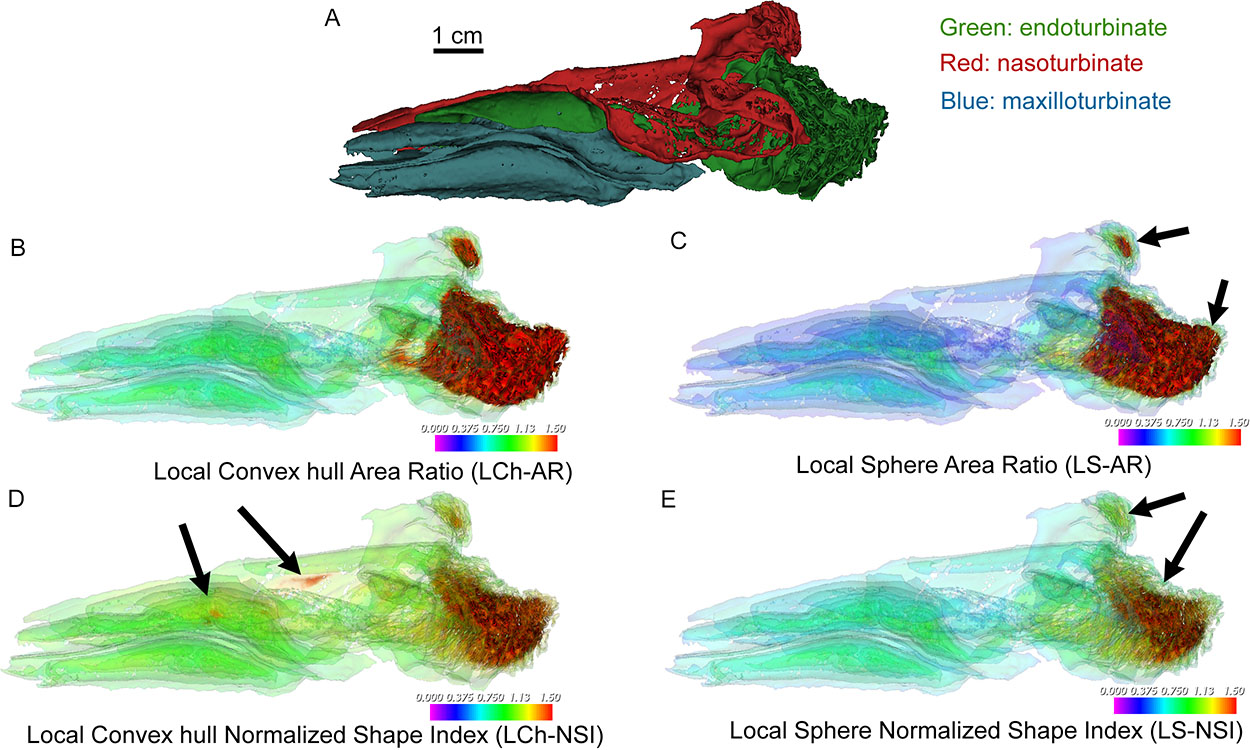
\includegraphics[scale=0.38]{images/11/complexity_example.jpg} 
	\caption{ 
Local complexity scalar computed in turbinate bones of \textit{Orycteropus afer}. \textbf{A}. Left endo, naso and maxillo turbinate bones viewed from the left side. Left-to-right: antero-posterior direction. Bottom-up: dorso-ventral direction. \textbf{B}: the Local Convex hull Area Ratio (LCh-AR) presents two advantages: no "border" artifacts, and no overestimation of complexity in flat-isolated regions.  \textbf{C}: the Local Sphere Area Ratio (LS-AR) tends to underestimate complexity at the outskirts of complex structures ("border artifacts", see black arrows).  \textbf{D}: the Local Convex hull Normalized Shape Index (LCh-NSI) tends to overestimate complexity is some very flat and isolated areas. See for instance the red areas in the center of the nasoturbinate and in the anterior part of the endoturbinate (black arrows). E: Local Sphere Normalized Shape Index (LS-NSI) presents no overestimation of complexity in flat-isolated regions, but tends to underestimate complexity at the outskirts of complex structures ("border artifacts", see black arrows). Image courtesy: Lionel Hautier and Mark Wright.
	}
\label{complexityexample}
\end{figure}

\section{Smooth active scalars for each selected surface}
It may happen that scalar values contain a lot of noise (see for instance the noisy results of the curvature computation in Fig. \ref{curvature_example}). In order to reduce noise and retrieve more biologically relevant information, scalars can be ``smoothed" in different ways (see \ref{smoothing_scalars_dialog}). Be aware that the obtained results depend very much on the size of the investigated local area for each vertex (based on direct neighbor vertices or on a much larger area), and on whether the new scalar value is computed as the average or as the median of the scalar values found for neighbor vertices (see Fig. \ref{smoothing_scalars_example}).

\begin{figure}
  \centering
  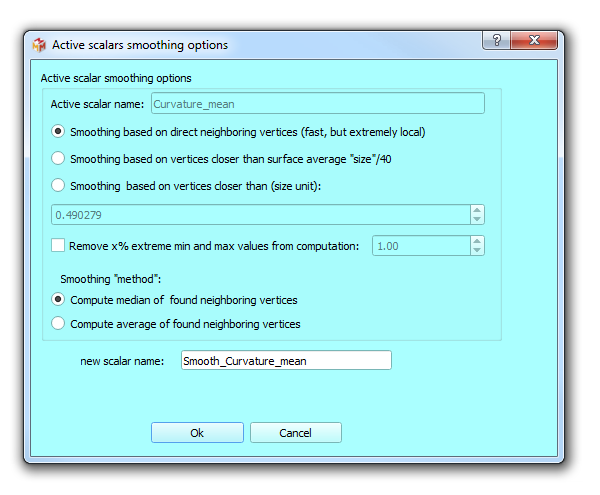
\includegraphics[scale=0.5]{images/11/scalar_smoothing_dialog.png} 
	\caption{ 
Scalar smoothing dialog. Smoothing can be computed using only direct neighbor vertices. A much larger area can also be investigated to produce a "smoothed" output. A percentage of extreme minimal and maximal values found can be excluded from the smoothing process. Also, the "smoothed" output can be computed as the average or as the median of the scalar values found for the neighbor vertices.
	}
\label{smoothing_scalars_dialog}
\end{figure}


\begin{figure}
  \centering
  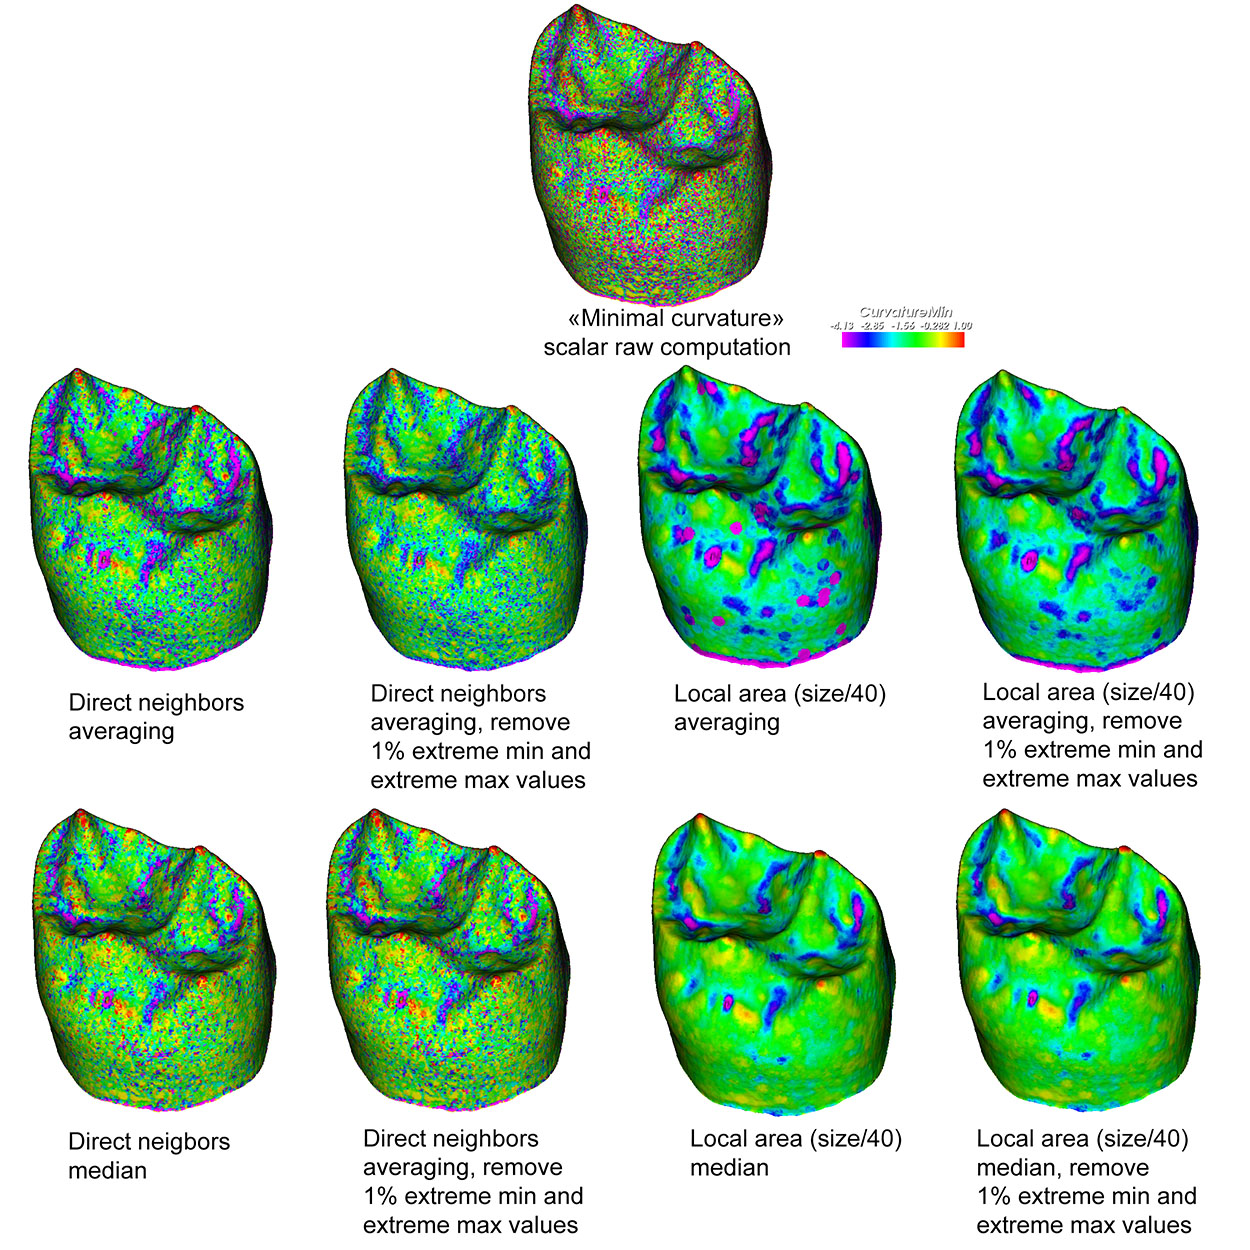
\includegraphics[scale=0.4]{images/11/scalar_smoothing_example.jpg} 
	\caption{ 
Smoothing scalars. Examples of 3D rendering of ``Min Curvature" scalars. \textbf{Top} : "raw" minimal curvature, which is extremely variable locally, and hard to interpret.  \textbf{Middle line}: averaging direct neighbors  or averaging scalar values on a much larger area give different results. See also how much averaging scalar values is sensitive with extreme min and max values. \textbf{Bottom line} : computing a median based upon direct neighbors  or upon scalar values found within a much larger area also give different results. The median smoothing "method"' is much less sensitive with extreme values (no difference seen when only 1\% of the most extreme min and max values are removed).  Specimen: enamel dentine junction (EDJ) of the second superior molar of a  Neolithic human of the necropolis of Gurgy (France). Image credit: Mona Le Luyer.	
	}
\label{smoothing_scalars_example}
\end{figure}


\section{Normalize or rescale active scalars for each selected surface}
It may be useful to normalize scalar values between 0 and 1, or to rescale them for different purposes. For instance, scalar normalization makes it possible to compare scalar arrays of different nature (and having very different min-max ranges) using a unique color scale ranging between 0 and 1. Also, in order to be able compare scalars such as bone thickness or enamel thickness variation between specimens of very different size, scalar normalization is a necessary step. The scalar normalization/rescale dialog is shown in Fig. \ref{normalization_dialog} p.\pageref{normalization_dialog}. An example of normalization of different scalars within a single surface is shown in Fig. \ref{normalization_example} p.\pageref{normalization_example}. An example of normalization of a single scalar in order to compare different specimens is shown in Fig. \ref{normalization_example2} p.\pageref{normalization_example2}.

\begin{figure}
  \centering
  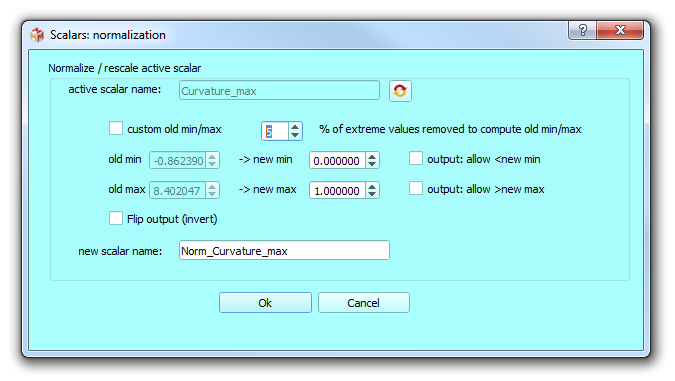
\includegraphics[scale=0.5]{images/11/normalization_dialog.png} 
	\caption{ 
Scalar normalization/rescale dialog. The "old min" and "old max" value represent by default the minimal and maximal value of the active scalars within \textbf{all} currently opened surfaces. After the scalar normalization/rescale has been performed, "old min" will have been set to "new min", "old max" will have been set to "new max", and scalar values in between "old min" and "old max" will range between "new min" and "new max" using a linear interpolation. "old min" and "old max" can be given other values than the real min and max of the active scalar via two options. \textbf{1)} a given percentage of extreme min and max values can be removed from the current active scalar values (sometimes only a few extreme "strange" values can give a wrong idea of the "real" extant of the range of a given scalar). \textbf{2)} if the "custom old min/max" option is checked, old min and old max values can be set to any value.  When one of these two options is used, the interpolated values produced may fall above "new max" or below "new min". Then you may decide whether you allow such "out of the range" values using the "allow < new min" and "allow > new max" options. If unchecked, interpolated values falling below "new min" will be set to "new min", and interpolated values falling above "new max" will be set to "new max". The "flip output" option will reverse the range of interpolated values between "new min" and "new max".
	}
\label{normalization_dialog}
\end{figure}

\begin{figure}
  \centering
  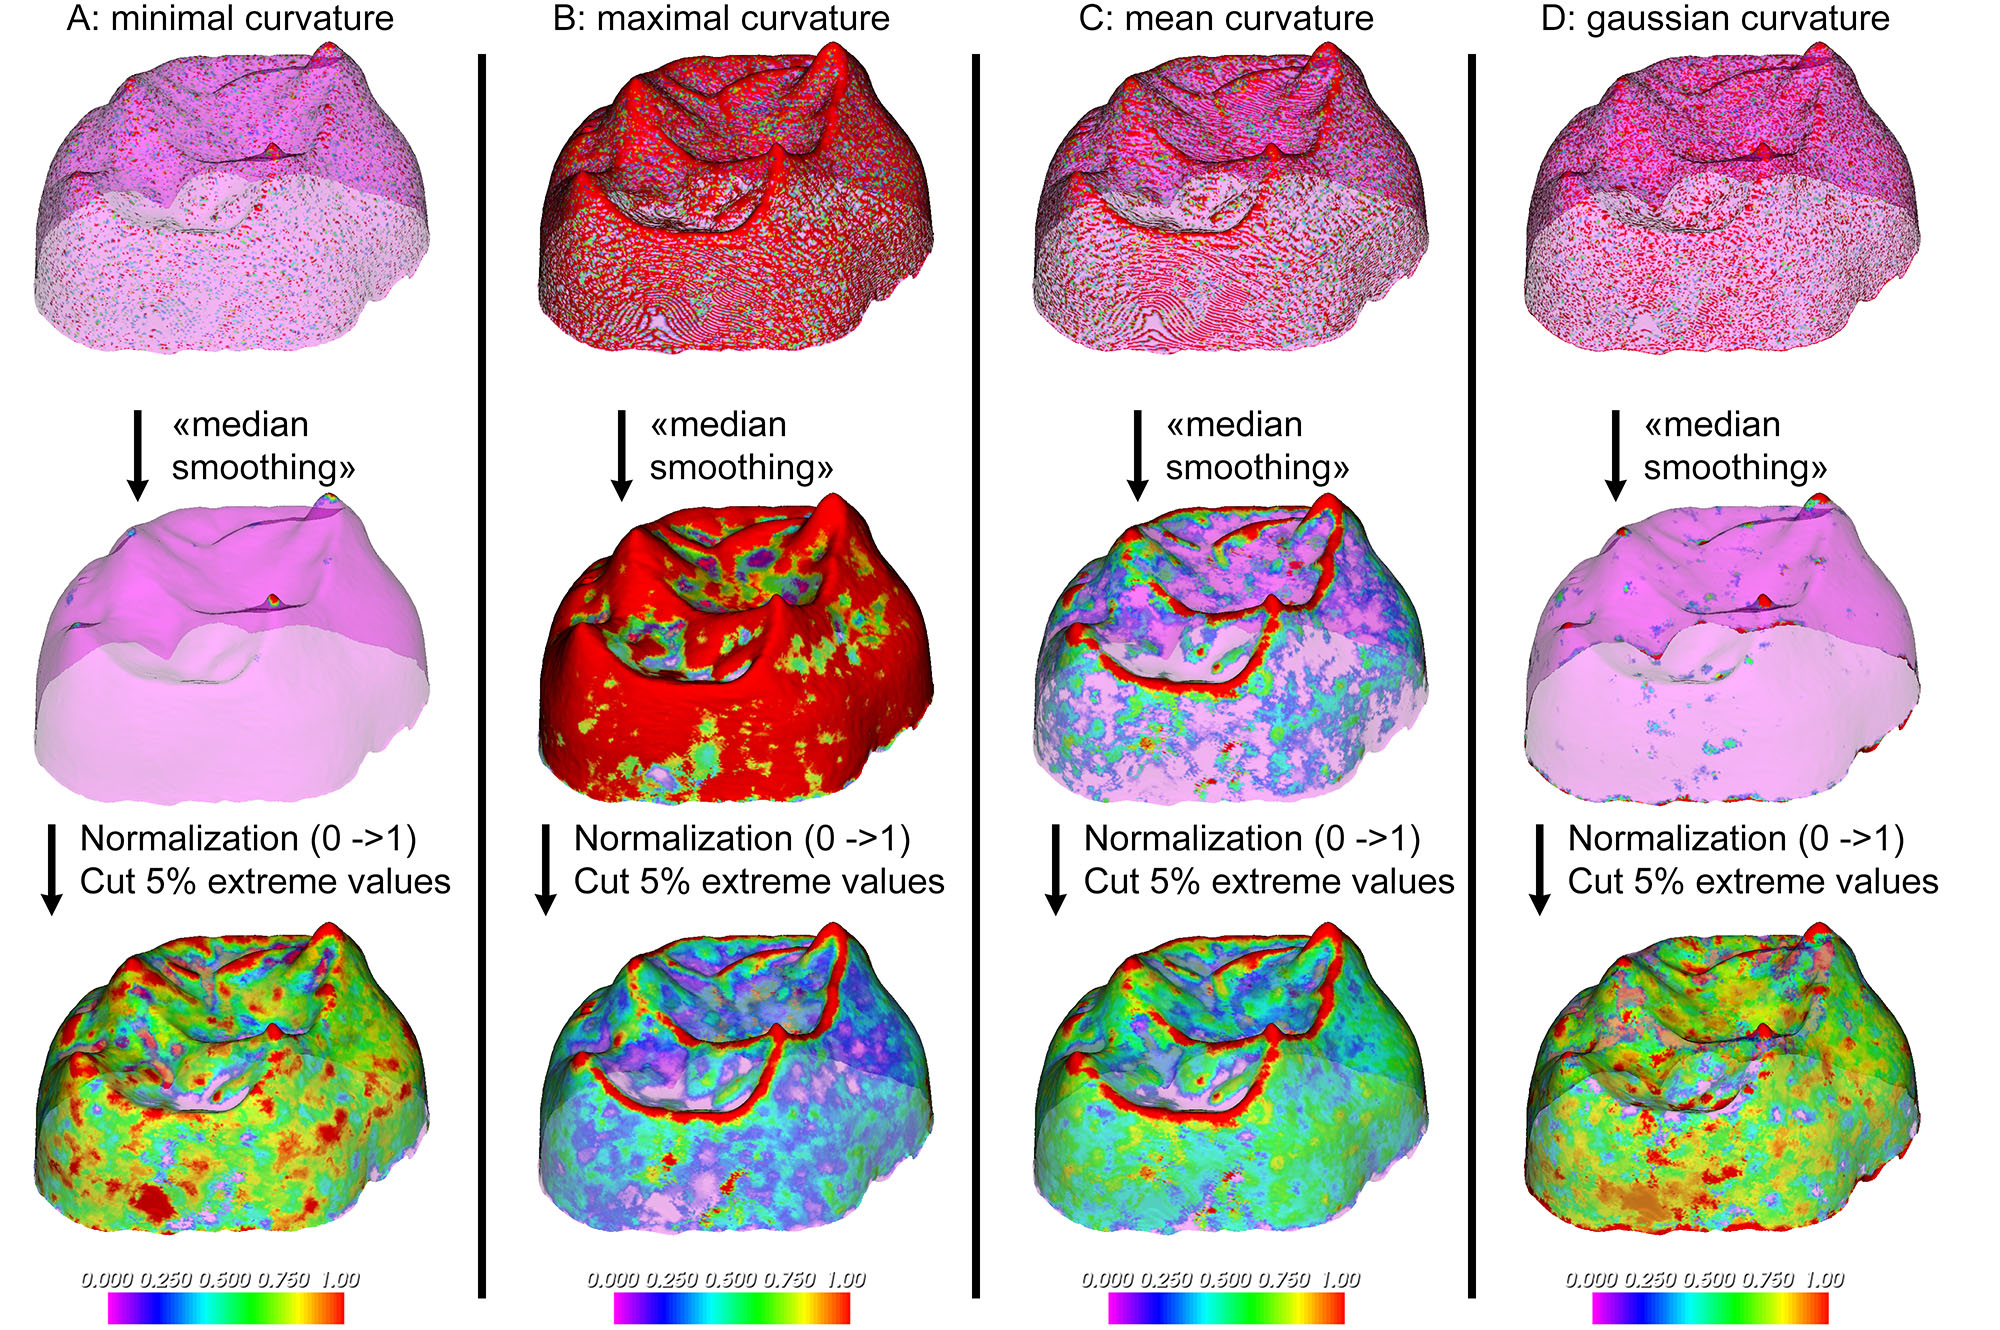
\includegraphics[scale=0.26]{images/11/normalization_example.jpg} 
	\caption{ 
Normalization of different scalars within the same specimen. All illustrations use the same color table, ranging between 0 and 1.  \textbf{A} : "Minimal curvature".  \textbf{B} : "Maximal curvature". \textbf{C} : "Mean curvature". \textbf{D} : "Gaussian curvature". Top line: "raw" 4 scalars, which all express a lot of noise. Middle line: the 4 same "smoothed"' scalars after a median filter has been used. Bottom line: the 4 same scalars after normalization. The 5\% most extreme minimal values and maximal values have been excluded from this normalization process, because they are clearly aberrant (most values range between -10 and 10 for all 4 raw scalars, but a few outliers have values above 10000 and below -10000). The visual output of the bottom line is easier to interpret. Specimen: enamel dentine junction (EDJ) of the second superior molar of a  Neolithic human of the necropolis of Gurgy (France). Image credit: Mona Le Luyer.	
	}
\label{normalization_example}
\end{figure}

\begin{figure}
  \centering
  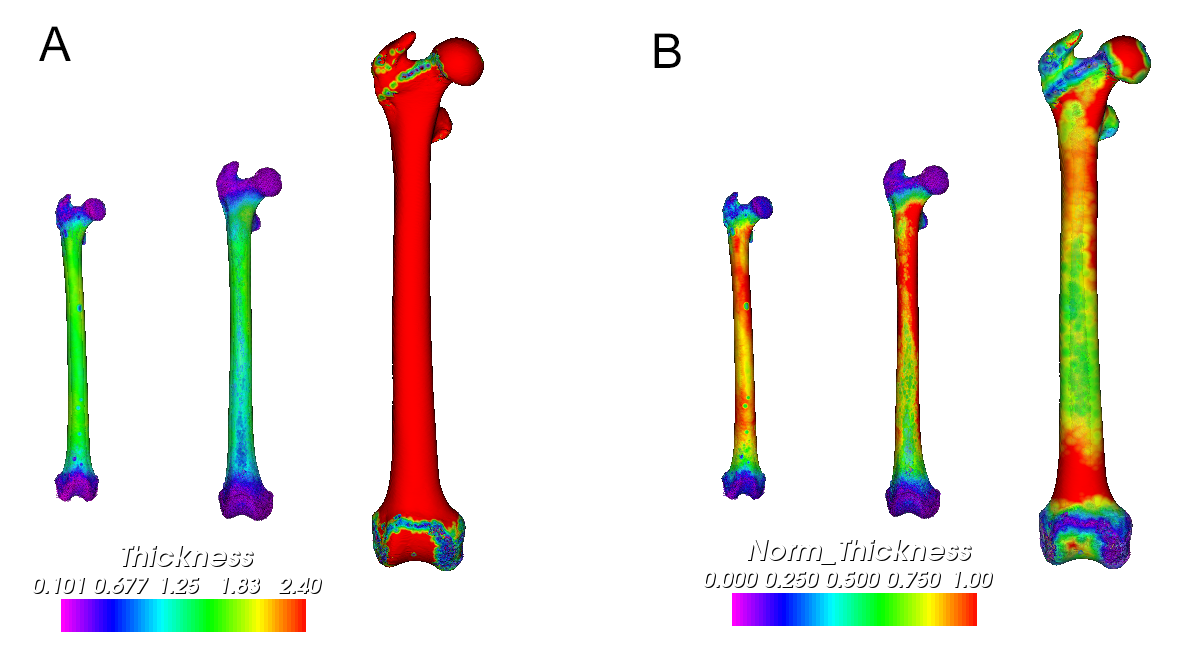
\includegraphics[scale=0.4]{images/11/normalization_example2.png} 
	\caption{ 
Normalization of a single scalar array in different specimens. From left to right in A and B: right femurs of \textit{Cercopithecus mona}, \textit{Erythrocebus patas}, \textit{Papio} sp.   \textbf{A}: "raw" bone thickness. See how bone thickness is much higher, generally speaking, for the femur of \textit{Papio sp.}, a relatively much larger primate than in the two others. This makes it hard to identify and compare variation of bone thickness for these three specimens. \textbf{B}: normalized bone thickness. Direct description and comparison between these three specimens is now possible. 	
	}
\label{normalization_example2}
\end{figure}
